		The given lines can be written  in vector form  as
\begin{align}
\begin{split}
	\vec{x} &= \myvec{1\\1\\0} + \kappa_1\myvec{2\\-1\\1},
	\\
	\vec{x} &= \myvec{2\\1\\-1} + \kappa_2\myvec{3\\-5\\2}
\end{split}
\label{eq:chapters/12/11/2/e11/lines}
\\
\begin{split}
	\vec{M} &= \myvec{2&3\\-1&-5\\1&2},
\vec{B} - \vec{A} = \myvec{1\\0\\-1}
\end{split}
\label{eq:chapters/12/11/2/e11/params}
\end{align}
%
Substituting the above in \eqref{eq:chapters/12/11/2/16/lsq/rank},
\begin{align}
\myvec{2&3&1\\-1&-5&0\\1&2&-1}
\xleftrightarrow[R_3 \leftarrow R_3 - \frac{1}{2}R_1]{R_2 \leftarrow R_2 + \frac{1}{2}R_1}
	\myvec{2&3&1\\[1ex]0&-\frac{7}{2}&\frac{1}{2}\\[1ex]0&\frac{1}{2}&-\frac{3}{2}}\\
\xleftrightarrow{R_3 \leftarrow R_3 + 7R_2}
	\myvec{2&3&1\\[1ex]0&-\frac{7}{2}&\frac{1}{2}\\[1ex]0&0&-10}
\end{align}
The rank of the matrix is 3. So the given lines are skew.
        From \eqref{eq:chapters/12/11/2/16/lsq/vec-eqn},
\begin{align}
\myvec{2&-1&1\\3&-5&2} \myvec{2&3\\-1&-5\\1&2}\bm{\kappa} &= \myvec{2&-1&1\\3&-5&2} \myvec{1\\0\\-1}\\
\implies \myvec{6&13\\13&38}\bm{\kappa} &= \myvec{1\\1}
\label{eq:chapters/12/11/2/e11/3}
\end{align}
The augmented matrix of the above equation \eqref{eq:chapters/12/11/2/e11/3} is given by,
\begin{align}
\myvec{6&13&\vrule&1\\13&38&\vrule&1}
\xleftrightarrow{R_2 \leftarrow R_2 - \frac{13}{6}R_1}
\myvec{6&13&\vrule&1 \\ 0&\frac{59}{6}&\vrule&-\frac{7}{6}}\\
\xleftrightarrow{R_1 \leftarrow R_1 - \frac{78}{59}R_2}
\myvec{6&0&\vrule&\frac{150}{59} \\ 0&\frac{59}{6}&\vrule&-\frac{7}{6}}
\end{align}
yielding
\begin{align}
	\myvec{\kappa_1\\-\kappa_2} &= \myvec{\frac{25}{59}\\[1ex]-\frac{7}{59}}
	\label{eq:chapters/12/11/2/e11/}
\end{align}
Substituting in \eqref{eq:chapters/12/11/2/e11/lines},
\begin{align}
\vec{x}_1 
= \frac{1}{59}\myvec{109\\34\\25},\,
\vec{x}_2 
= \frac{1}{59}\myvec{139\\24\\-45}.
\end{align}
The minimum distance between the lines is given by,
\begin{align}
\norm{\vec{x}_2-\vec{x}_1} &= \norm{\frac{1}{59}\myvec{30\\-10\\-70}}
= \frac{10}{\sqrt{59}}
\end{align}
See Fig. 
	\ref{fig:chapters/12/11/2/e11/}.
\begin{figure}[H]
\centering
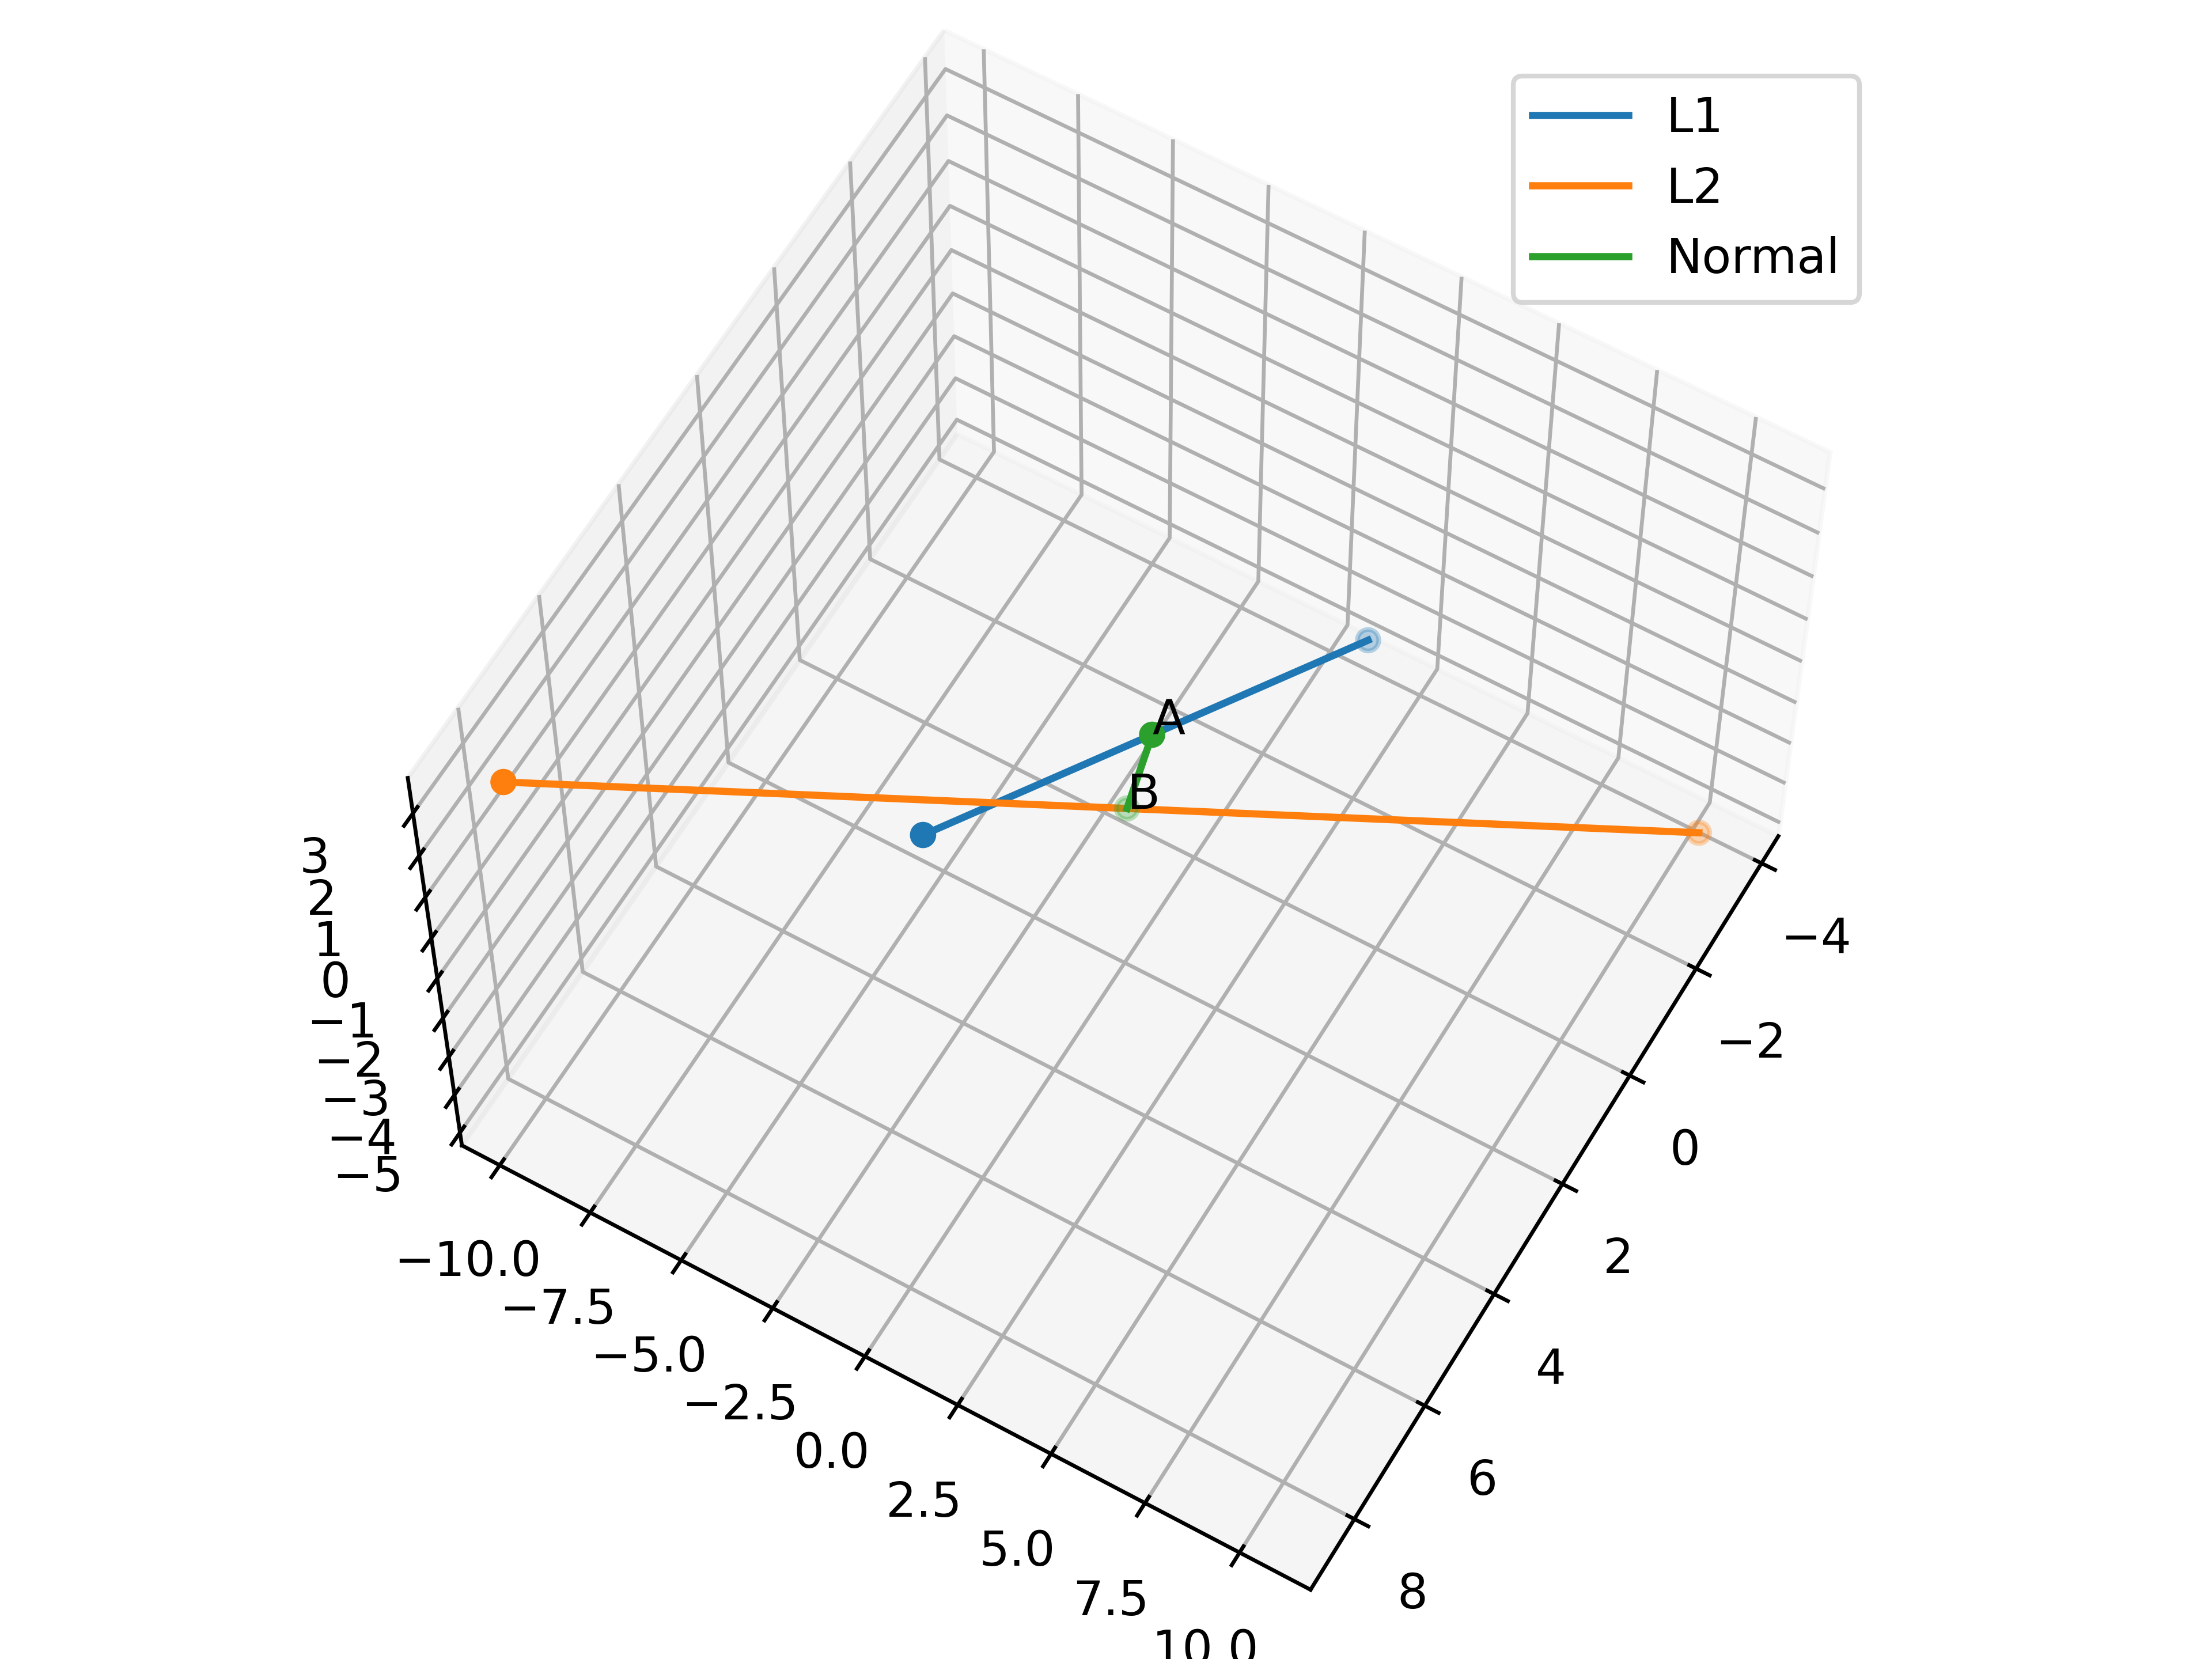
\includegraphics[width=0.75\columnwidth]{chapters/12/11/2/e11/lsq/figs/skew.png}
\caption{}
	\label{fig:chapters/12/11/2/e11/}
\end{figure}
